\section{Early Validation}
\label{sec:evaluation}

%In this section we present the evaluation of \parikshan. 
%The key questions facing us were:
%\begin{itemize}
%  \item How can \parikshan be used in the real world? 
%  \item Does the test container faithfully represent the execution and the state of the production container? 
%     \item How does cloning the container effect the performance of the production container?
%     \item How long of a testing-window do we have? 
%   \item How does running tests in the test-container effect the performance of the production container?
%\end{itemize}

%In order to answer these questions, we separated our evaluation in looking at two different stages: cloning stage, time-window analysis.

%\subsection{Cloning: Micro-Benchmarks}
%\label{sec:performance}

\begin{table}[ht]
  \centering
    \begin{tabular}{ | p{1.8cm} | l | l | l | l |}
    \hline
    \textbf{Modes} & \multicolumn{2}{|c|}{\textbf{Internal Mode}} & \multicolumn{2}{|c|}{\textbf{External Mode}}\\\hline
    \textbf{ } & \textbf{Cloning} & \textbf{Hog+Cloning} & \textbf{Cloning} & \textbf{Hog+Cloning} \\ \hline
    \hline
    \textbf{Throughput} & --  & 1509 req/s & --  & 625\\ \hline
    \hline
    \textbf{Suspend + Dump} & 0.49 & 0.46 & 0.10  & 0.10\\ \hline
    \textbf{Pcopy } & 0.22  & 0.27 & 0.44  & 0.39\\ \hline
    \textbf{Copy Dump } & 0.62  & 0.64 & 0.28  & 0.31 \\ \hline
    \textbf{Undump} & 1.33  & 1.53 & 0.84 & 1.03 \\ \hline 
    %\textbf{--------------} & --- & --- & --- & --- & --- & --- & --- & --- & --- \\ 
    \hline
    \textbf{Suspend Time} & 2.66 & 2.91 & 1.67 & 1.83 \\ \hline
    \end{tabular}
    \caption{Performance of container cloning suspend time in external vs internal modes, when running httperf webserver hog workload.
      The hog processes 1601 req/s without any cloning in the internal mode, and 675 req/s in the external mode}
\label{table:clonePerf}
\end{table}

%The profile of the cloning operation can be divided in 4 stages: 
%(1) Suspend \& Dump: this is the time taken to suspend the container, 
%(2) Pcopy after suspend: which does the rsync after the suspend of the file system of the container, 
%(3) Copy Dump File: which copies the process state, and finally 
%(4) Undump and Resume: which is the time taken to resume the containers. 

\noindent \textbf{ Q1: How does cloning impact production systems and how fast is cloning?  }
In Table \ref {table:clonePerf}, we show the suspend times when cloning a production container (webserver) that is idle vs. a container which is running an Apache hog benchmark \cite{httperf} on it. 
The first column gives the average performance of the cloning operation without any hog operation running on it.  
An idle or a container with minimal processing is cloned relatively fast: 2.66 seconds on the idle container. 
We then tried to run an Apache hog to make a baseline of Apache's performance without cloning, and found that a page fetch gave us a throughput of 1601 req/s (internal mode). Then we tried to do cloning of the same container while running the hog, and found minimal change (1509 req/s) in the performance of the hog, and very little impact on the suspend time of live cloning.
The key thing to note in these experiments was that we \textbf{did not have any connection failure or connection refused, and only a slight decline in the throughput during the cloning operation}. 
At the application layer, the TCP packet drops are hidden as packets are resent from within the TCP protocol.
%To further investigate the tcp packet dropping, we ran an iperf\cite{iperf}( a tool to measure tcp benchmark) server while cloning the production container. 
%We were indeed able to observe packet dropping for about 2 seconds in the iperf client, however, the important point to note is that there were no requests dropped for the application while doing cloning. 
\iffalse
\begin{figure*}[t]
	\begin{center}
		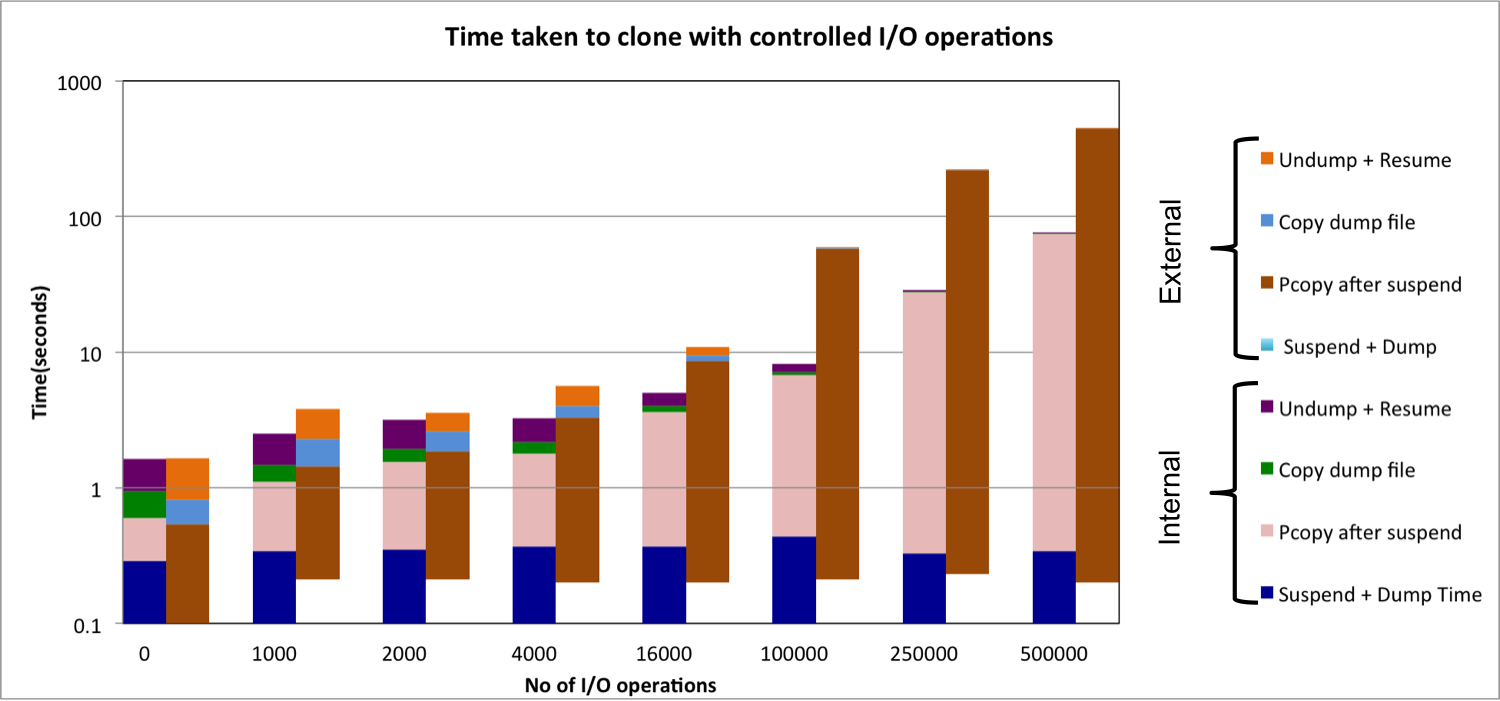
\includegraphics[width=1\textwidth]{figs/fioResult.png}
		\caption{Comparison between cloning between the internal vs external mode, while continuously increasing the file write operations to disk}
		\label{fig:fioResults}
	\end{center}
\end{figure*}
\fi
%As explained earlier, the cloning process can be divided into two parts: an rsync operation which does an ``pre-copy'' of the VM, and a follow-up rsync operation while the target container is suspended, to make sure that both the production and test containers have the exact same state.
%The idea is to reduce the time taken to suspend the production container, so that it has minimal effect on the user.

\noindent \textbf{ Q2: What factors effect cloning performance? }
The main factor that effects suspend time is the number of ``dirty pages'' in the suspend phase, which have not copied over in the pre-commit rsync operation.
%Naturally, the number of write operations in the container while cloning the container, will increase the number of dirty pages, and increase the time of the suspend operation.
%To understand the effect that I/O operations have on the cloning operation, we ran a controlled experiment gradually increasing the number of I/O writes and writes. 
We use fio(flexible io tool for linux)\cite{fio}, to increase the number of I/O operations while doing cloning. 
%Specifically, we do random-write operations of a 500MB file with fixed i/o bandwidth rates.
%As shown in figure \ref{fig:fioResults}, i
In our experiments with a read intensive workload, the suspend time was about 3-4 seconds, with upto 2-3 Mbps of read I/O. 
In essence, we found that read operations do not really impact the performance of our cloning. 
On the other hand for write operations, cloning has minimal impact for write I/O bandwidths of about 100Kbps - 150 Kbps operations. 
However, it increased rapidly beyond that. Thus, the increased cloning time confirmed our intuition that the cloning operation will be impacted when running a write I/O intensive application.
.
%Here we also compare the performance of cloning in the internal mode vs the external mode, while showing the time taken in various stages of cloning.
%While for lower I/O operations, the performance of both were similar, as we go higher, the external mode which uses the network to transfer the dirty pages during the cloning operations becomes a bottleneck. 
%The internal mode is much faster as both the production and test-container are hosted in the same physical device, so they have a much higher bandwidth between them.
%We can also see that the majority of the time is spent in pcopy after suspend, which is doing the copy of the dirty bits after suspend, especially for higher I/O's the other operations become negligible in comparison.
We would like to point out here, that most SOA application are usually read or CPU intensive operations, and several studies have shown live migration performance to be acceptable\cite{vmperformance} for most application SLA's. 
To conclude, we validated that live cloning generally takes less than two seconds  and is not disruptive to application clients (there is no loss of service visible). 
However, in high I/O write intensive workloads, the amount of time taken to clone can reach one or two minutes.
In such cases, we did observe retries and the performance of the server did suffer. 
Rate-limiting in the proxy can possibly be applied as a mitigating mechanism to allow for reduced suspend time in cloning. 
Alternatively some migration approaches use many more iterations or network-page faults, to reduce the suspend time further. For sake of brevity we do not discuss them here.

\iffalse
\textbf{Case-Study: } we debugged some real bugs such as mysql bug 18511 \cite{mysqlbug}, and did performance profiling of PetStore a 3 tier J2EE e-commerce system. 
We were able to increase the instrumentation sufficiently to debug the system within the test-container, by first doing a function level execution trace, and then adding a breakpoint at suspiciously long executions.
Using debugging and instrumentation tools, we were able to localize the bug to a highly non-optimal string matching for japanese, and chinese characters.
Simultaneously we observed no performance degradation in the production system.
%Current research in live migration has looked into further decreasing the sync time by doing active migration, and trigger page fault for the dirty bits which were not copied over.
%This is a similar to a copy-on-write method, that could possibly reduce our suspend time.
%In the interest of time, we have not explored faster means of live cloning, but aim to do so in our future work.
%However, it would impact, the overall performance of both systems as it would do the rsync operation for a much longer time-period.
\fi
\iffalse
\subsection{Time-Window Size Evaluation}
\label{sec:timewindowPerformance}

As explained in section \ref{sec:timewindowPerformance} if the overhead of the test-container is too high, the buffer may overflow.
This indirectly means that the test-container and the production-container are potentially out of sync.
In our current design we re-initiate the test-container by cloning again, and we call the time taken to reach a buffer overflow the "time-window" for the test-container.
As explained earlier, the size of this test-container, depends both on the overhead of the "test"/"instrumentation", as well as the incoming workload.

In this section we evaluate the testing window size using varying amounts of instrumentation, and the workload.
For the purpose of this evaluation, we keep a fixed buffer size. 
First we use a controlled workload rate, and gradually increase the overhead, then we use another scenario, where we keep the try to keep the same overhead, and try to increase the workload.
We also use real-world network packet capture data, to simulate a realistic workload and gradually increase the overhead there

\texttt{Nipun's note: This section still needs to be completed, I'm finishing up some of the results, before I can generate the charts}

\subsection{Overhead while Running tests}
\label{sec:overhead}

One of the most important goals of using \parikshan is to allow debugging without having any overhead on the actual application.
In this section we verify that this goal of \parikshan holds true i.e. debugging in the sandbox-container, does not effect the performance container. 
To understand the effect we ran some tests on our cloned container, with an independent cpu hog (infinite while loop with sleep) running within the test.
We gradually increased the amount of cpu being used by the cpu hog and found that while in the external mode there is no effect on the performance of the production container, in the internal mode at higher cpu hog percentages, the throughput of the production container is reduced.
This was an expected result, as the production container and test-container time share resources on the same machine, whereas in the external mode, they are completely isolated.
However, it is to be noted, that most debugging scenarios are unlikely to be cpu hogs, and if resource management in the container level is done properly, the containers in the internal-mode can be largely isolated from each other.

\fi
